\subsection{Experimentos}

\textbf{En esta sección se presentan cuatro experimentos diseñados para evaluar sistemáticamente el rendimiento, eficiencia y aplicabilidad de las MH en comparación con los métodos de GD para el entrenamiento de redes neuronales profundas}. Los experimentos abordan aspectos complementarios que, en conjunto, proporcionan una visión integral del comportamiento de ambos enfoques en diversos escenarios.

\textbf{El primer experimento analiza si existen diferencias estadísticamente significativas en el rendimiento de redes MLP entrenadas con MH según el tipo de tarea} (clasificación vs. regresión). Utilizando conjuntos de datos de complejidad equiparable y aplicando rigurosos tests estadísticos, se evalúa el rendimiento relativo de SHADE-ILS frente a AdamW en ambos tipos de tareas.

\textbf{El segundo experimento profundiza en los factores que más influyen en la pérdida de rendimiento en tareas de clasificación}, tanto en MLPs como en ConvNets. Mediante un análisis de dependencias parciales, se examina cómo la cantidad de ejemplos, la complejidad del conjunto de datos y el número de parámetros del modelo afectan al rendimiento predictivo de los modelos entrenados con ambos tipos de optimizadores (MH y GD).

\textbf{El tercer experimento se centra en analizar los tiempos de ejecución durante el entrenamiento con MH en comparación con el GD}. Este análisis desglosado permite comprender no solo las diferencias absolutas en tiempo, sino también los factores que más impactan en la eficiencia computacional de cada enfoque.

\textbf{Finalmente, el cuarto experimento evalúa el rendimiento de propuestas híbridas propias, específicamente SHADE-GD y SHADE-ILS-GD, que combinan elementos de MH y GD}. Este análisis comparativo determina si estos enfoques híbridos logran capitalizar las fortalezas de ambas técnicas y superar sus limitaciones individuales.




\subsubsection{Experimento 1: Análisis de diferencias en el rendimiento de MLPs entrenados con MH según el tipo de tarea}


\begin{table}[]
\resizebox{\textwidth}{!}{\begin{tabular}{|c|c|ccc|ccc|c|}
\hline
\multirow{2}{*}{Conjunto} & \multirow{2}{*}{Capas} & \multicolumn{3}{c|}{ADAMW}                                        & \multicolumn{3}{c|}{SHADE-ILS}                                         & \multirow{2}{*}{\textbf{Dif$_{rel}$}} \\ \cline{3-8}
                          &                        & \multicolumn{1}{c|}{Train}  & \multicolumn{1}{c|}{Test}  & Metric & \multicolumn{1}{c|}{Train}  & \multicolumn{1}{c|}{Test}   & Metric     &                                       \\ \hline
\multirow{4}{*}{BCW}      & 1                      & \multicolumn{1}{c|}{0.190}  & \multicolumn{1}{c|}{0.108} & 0.960  & \multicolumn{1}{c|}{0.073}  & \multicolumn{1}{c|}{0.142}  & 0.970      & \textbf{0.010}                        \\ \cline{2-9} 
                          & 2                      & \multicolumn{1}{c|}{0.140}  & \multicolumn{1}{c|}{0.041} & 0.980  & \multicolumn{1}{c|}{0.063}  & \multicolumn{1}{c|}{0.350}  & 0.932      & \textbf{-0.049}                       \\ \cline{2-9} 
                          & 5                      & \multicolumn{1}{c|}{0.115}  & \multicolumn{1}{c|}{0.026} & 1.000  & \multicolumn{1}{c|}{0.055}  & \multicolumn{1}{c|}{0.475}  & 0.890      & \textbf{-0.110}                       \\ \cline{2-9} 
                          & 11                     & \multicolumn{1}{c|}{0.112}  & \multicolumn{1}{c|}{0.094} & 0.971  & \multicolumn{1}{c|}{0.098}  & \multicolumn{1}{c|}{0.491}  & 0.903      & \textbf{-0.07}                        \\ \hline
\multirow{4}{*}{WQC}      & 1                      & \multicolumn{1}{c|}{0.970}  & \multicolumn{1}{c|}{2.172} & 0.436  & \multicolumn{1}{c|}{1.098}  & \multicolumn{1}{c|}{1.235}  & 0.201      & \textbf{-0.539}                       \\ \cline{2-9} 
                          & 2                      & \multicolumn{1}{c|}{0.873}  & \multicolumn{1}{c|}{3.177} & 0.500  & \multicolumn{1}{c|}{1.078}  & \multicolumn{1}{c|}{1.340}  & 0.167      & \textbf{-0.666}                       \\ \cline{2-9} 
                          & 5                      & \multicolumn{1}{c|}{0.770}  & \multicolumn{1}{c|}{3.833} & 0.606  & \multicolumn{1}{c|}{0.963}  & \multicolumn{1}{c|}{1.405}  & 0.167      & \textbf{-0.724}                       \\ \cline{2-9} 
                          & 11                     & \multicolumn{1}{c|}{0.940}  & \multicolumn{1}{c|}{3.873} & 0.607  & \multicolumn{1}{c|}{1.137}  & \multicolumn{1}{c|}{1.509}  & 0.167      & \textbf{-0.725}                       \\ \hline
\multirow{4}{*}{WQR}      & 1                      & \multicolumn{1}{c|}{0.475}  & \multicolumn{1}{c|}{0.972} & -0.012 & \multicolumn{1}{c|}{0.611}  & \multicolumn{1}{c|}{0.970}  & -1.988     & \textbf{-164.667}                      \\ \cline{2-9} 
                          & 2                      & \multicolumn{1}{c|}{0.430}  & \multicolumn{1}{c|}{1.126} & 0.072  & \multicolumn{1}{c|}{0.551}  & \multicolumn{1}{c|}{0.826}  & -2.491     & \textbf{-35.597}                      \\ \cline{2-9} 
                          & 5                      & \multicolumn{1}{c|}{0.390}  & \multicolumn{1}{c|}{1.180} & 0.236  & \multicolumn{1}{c|}{0.589}  & \multicolumn{1}{c|}{0.724}  & -983.152   & \textbf{-4166.898}                    \\ \cline{2-9} 
                          & 11                     & \multicolumn{1}{c|}{0.377}  & \multicolumn{1}{c|}{2.162} & 0.133  & \multicolumn{1}{c|}{0.601}  & \multicolumn{1}{c|}{0.734}  & -79529.602 & \textbf{-597967.932}                  \\ \hline
\multirow{4}{*}{BHP}      & 1                      & \multicolumn{1}{c|}{84.429} & \multicolumn{1}{c|}{6.332} & 0.790  & \multicolumn{1}{c|}{10.048} & \multicolumn{1}{c|}{7.549}  & 0.576      & \textbf{-0.271}                       \\ \cline{2-9} 
                          & 2                      & \multicolumn{1}{c|}{55.283} & \multicolumn{1}{c|}{4.577} & 0.832  & \multicolumn{1}{c|}{9.560}  & \multicolumn{1}{c|}{4.648}  & 0.746      & \textbf{-0.103}                       \\ \cline{2-9} 
                          & 5                      & \multicolumn{1}{c|}{94.640} & \multicolumn{1}{c|}{3.511} & 0.847  & \multicolumn{1}{c|}{13.594} & \multicolumn{1}{c|}{14.555} & -0.187     & \textbf{-1.221}                       \\ \cline{2-9} 
                          & 11                     & \multicolumn{1}{c|}{54.540} & \multicolumn{1}{c|}{3.268} & 0.853  & \multicolumn{1}{c|}{43.183} & \multicolumn{1}{c|}{26.794} & -97.404    & \textbf{-115.190}                     \\ \hline
\end{tabular}}
\caption[Resultados del entrenamiento y evaluación de los modelos asociados al primer experimento]{Resultados del entrenamiento y evaluación de los modelos asociados al primer experimento. A partir de estos, intentamos averiguar, a través del test de los rangos con signo de Wilcoxon, si existe una diferencia estadísticamente significativa en el rendimiento de modelos entrenados con MH según el tipo de tarea. Los conjuntos de datos usados son BCW y WQC para clasificación y BHP y WQR para regresión. Estas tareas tienen una complejidad similar dos a dos (BCW-BHP y WQC-WQR). Los MLP, de entre 1 y 11 capas ocultas, son entrenados usando SHADE-ILS como técnica MH y ADAMW como optimizador basado en GD. Como métricas, se usa \textbf{\textit{Balanced Accuracy}} en clasificación y \emph{\textbf{R$^2$}} en regresión. La comparación, realizada de manera relativa observando el rendimiento de los modelos entrenados con MH en relación con su análogo entrenado con GD, no arroja resultados concluyentes.}
\label{tab:exp1}
\end{table}

En este experimento, planteamos la hipótesis de que \textbf{los modelos MLP entrenados con MH presentan diferencias significativas en su rendimiento según el tipo de tarea} (clasificación o regresión). En particular, investigamos si estas diferencias se deben a la naturaleza de la tarea, más que a factores como la complejidad del problema o la arquitectura de la red. Esta hipótesis \textbf{se fundamenta en evidencias experimentales}, como los resultados presentados en la Tabla \ref{tab:exp1}, que sugieren un comportamiento diferenciado en el rendimiento de SHADE-ILS según el tipo de tarea, a diferencia de lo que ocurre con AdamW.

En los conjuntos de datos de clasificación (BCW y WQC), se observa que AdamW tiende a obtener un mejor desempeño en términos de métrica \textit{Balanced Accuracy} en comparación con SHADE-ILS a medida que aumenta la profundidad de la red. Por ejemplo, en el conjunto WQC con 11 capas, la diferencia relativa (Dif$_{rel}$) es de -0.725, lo que indica una ventaja significativa a favor de AdamW. Por otro lado, en los conjuntos de regresión (BHP y WQR), el comportamiento es más errático y con diferencias relativas mucho más extremas. Destaca especialmente el caso de WQR con 11 capas, donde la Dif$_{rel}$ alcanza valores negativos elevados (-597967.932), lo que sugiere que SHADE-ILS tiene dificultades para optimizar redes profundas en tareas de regresión.

Estos resultados nos llevan a plantear la hipótesis de que el rendimiento de los modelos entrenados con MH podría estar influenciado de manera significativa por el tipo de tarea. Mientras que para tareas de clasificación SHADE-ILS muestra una degradación de rendimiento más gradual, en tareas de regresión se observan desviaciones mucho más marcadas, especialmente con arquitecturas más complejas.


Para realizar esta comparación, entrenaremos en cuatro conjuntos de datos tabulares: dos de clasificación (BCW y WQC) y dos de regresión (BHP y WQR), agrupados por complejidad (BCW-BHP y WQC-WQR), a través de los optimizadores MH SHADE y SHADE-ILS, y los basados en GD AdamW y RMSProp, ya que son los que arrojan mejores resultados. Utilizamos arquitecturas de MLP con 1, 2, 5 y 11 capas ocultas. 

Como las métricas usadas para clasificación y regresión son distintas y no son comparables directamente, debemos establecer la comparación en términos relativos. Observamos que los modelos entrenados con GD no muestran diferencias en el rendimiento dependiendo de la tarea, y analizaremos la diferencia relativa de rendimiento entre MH y GD para cada tipo de tarea, realizando el promedio entre los dos optimizadores utilizados de cada tipo (SHADE y SHADE-ILS; AdamW y RMSProp). Si las diferencias relativas son estadísticamente significativas, es decir, si la diferencia de rendimiento entre MH y GD para cada tipo de tarea es distinta, entonces concluiremos que los modelos entrenados con MH muestran diferente rendimiento dependiendo del tipo de tarea. Definimos la fórmula


$$Dif_{rel} = \frac{Metric_{MH}-Metric_{GD}}{|Metric_{GD}|}.$$


A partir de esta fórmula, obtenemos dos muestras: las diferencias relativas para clasificación y las diferencias relativas para regresión. El objetivo es determinar si existe una diferencia estadísticamente significativa entre ambas. Como son muestras dependientes, deberemos utilizar bien el t-test para muestras pareadas o bien el test de Wilcoxon de los rangos con signos. La elección de uno u otro dependerá de si las muestras siguen una distribución normal o no, utilizando t-test en el caso afirmativo y Wilcoxon en el contrario.

En primer lugar, verificamos la normalidad de las muestras mediante la prueba de Shapiro-Wilk, donde la hipótesis nula establece que las diferencias relativas siguen una distribución normal. Obtenemos un p-valor de 0.003, por debajo de los niveles de significacnia habituales (0.05, 0.01) lo que implica el rechazo de la hipótesis nula y confirma que las muestras no siguen una distribución normal.

\begin{table}[]
\centering
\begin{tabular}{|c|c|c|}
\cline{1-3}
                                Test                                                                   & Estadístico & P-valor        \\ \hline
\multicolumn{1}{|c|}{Shapiro-Wilk}                                 & 0.635       & \textbf{0.003}                      \\ \hline
\multicolumn{1}{|c|}{Wilcoxon rangos con signo} & 6.000       & \textbf{0.023}                       \\ \hline
\end{tabular}
\caption[Resultado de los tests estadísticos llevados a cabo durante el primer experimento]{Resultado de los tests estadísticos llevados a cabo durante el primer experimento. Para medir objetivamente que no haya diferencia de rendimiento según el tipo de tarea para modelos de la familia MLP entrenados con MH, hemos medido el rendimiento relativo en comparación a un modelo análogo entrenado con GD. Aplicamos el test Shapiro-Wilk a la muestra resultante de las medidas relativas\footnote{Realmente se lo aplicamos a una única muestra, que resulta de la diferencia de las muestras de regresión y clasificación.}, con la hipótesis nula siendo que la muestra sigue una distribución normal. Al comprobar que no lo hace, y como se trata de muestras dependientes, aplicamos el test de Wilcoxon de los rangos con signos, con la hipótesis nula siendo que no hay diferencia de rendimiento entre clasificación y regresión en modelos MLP entrenados con MH. Obtenemos un p-valor que no nos da una evidencia suficiente para rechazar la hipótesis nula.}
\label{tab:stats}
\end{table}

En consecuencia, aplicamos la prueba no paramétrica de Wilcoxon.  La hipótesis nula en este caso establece que no existen diferencias en el rendimiento relativo al GD entre las tareas de clasificación y regresión. \textbf{Obtenemos un p-valor de 0.023, que es inferior al nivel de significancia habitual de 0.05, lo que nos permite rechazar la hipótesis nula. Esto sugiere que existen diferencias significativas en el rendimiento relativo al GD entre ambas tareas.} Sin embargo, estos resultados parecen bastante sensibles a los optimizadores incluidos en el experimento, por lo que se deben tomar las conclusiones con cautela.





\subsubsection{Experimento 2: Evaluación de los factores que más afectan a la pérdida de rendimiento en tareas de clasificación, tanto en MLPs como en ConvNets}

La hipótesis que planteamos en este segundo experimento es que\textbf{ la pérdida de rendimiento en modelos de clasificación, ya sean entrenados con MH o con GD, está fuertemente influenciada por la cantidad de ejemplos en el conjunto de datos, la complejidad del conjunto de datos y el número de parámetros del modelo}. Específicamente, esperamos que un menor número de ejemplos y un aumento en la complejidad del conjunto de datos o en el número de parámetros del modelo conduzcan a un deterioro significativo en el rendimiento predictivo.

Hemos seleccionado tres factores, comunes a cualquier tarea, que pueden influir notablemente: cantidad de ejemplos del conjunto de datos, complejidad del conjunto de datos y número de parámetros del modelo. Para esta tarea vamos a analizar los factores que acabamos de proponer a través de un análisis de dependencias parciales, con el fin de aislar la contribución de cada factor al rendimiento del modelo.

El análisis de dependencias parciales es una técnica utilizada en aprendizaje automático para interpretar modelos predictivos. Permite visualizar la relación entre una o más características de entrada y la salida del modelo, manteniendo fijas otras variables para aislar su efecto. Nosotros no lo usaremos sobre el modelo en sí, sino que tomaremos como características los factores que queremos evaluar, como desarrollaremos más adelante, y al aplicarlo obtendremos información sobre la importancia de cada factor en la salida del modelo. Si la gráfica es creciente indica un impacto positivo; si es decreciente el impacto es negativo, y si es no lineal indica relaciones complejas, como que esa variable dependa de otras. Cuanto mayor sea la pendiente de la gráfica, mayor es la relación de la variable con la salida.

La valoración de la métrica que usemos para medir el rendimiento será dependiente de la tarea. No es lo mismo obtener un 50\% de \textit{accuracy} en CIFAR-10G, que al haber 10 clases no tiene por que ser un mal rendimiento, que obtener ese dato en BCW donde solo hay dos clases a clasificar, lo que indicaría un rendimiento parejo al de un clasificador aleatorio. Por tanto, vamos a quitar el sesgo del número de clases, y \textbf{como métrica de rendimiento vamos a usar el \textit{accuracy} obtenido en relación al del clasificador aleatorio para esa tarea.} \textbf{Denominaremos a dicha métrica RA, con el valor de 0 simbolizando un rendimiento igual al del clasificador aleatorio}. Un valor negativo indica que el rendimiento empeora con respecto al clasificador aleatorio, y un valor positivo indica que mejora. Un valor de uno equivaldría a un \textit{accuracy} de 1. En WQC consideraremos solo 6 clases a predecir ya que es el número de clases que contienen ejemplos dentro del conjunto de datos. 

$$RA = \frac{balanced\_accuracy - accuracy_{clasificador\_aleatorio}}{accuracy_{clasificador\_aleatorio}}.$$

Compararemos el rendimiento usando AdamW y RMSProp como optimizadores basados en GD, ya que son los que mejor resultado consiguen en las tareas correspondientes, con SHADE y SHADE-ILS como técnicas MH. Para obtener diferentes valores de los tres factores mencionados, usaremos 5 conjuntos de datos: BCW,  WQC, MNIST, F-MNIST y CIFAR-10G. Entrenaremos los modelos LeNet5, ResNet15 y ResNet57 en tareas con imágenes y MLP capas 1,2,5,11 para tareas tabulares. 


Para un correcto análisis vamos a asignar valores numéricos que representen a los factores que hemos mencionado. Englobamos un conjunto de datos, según el número de ejemplos, en tres valores: pocos (1), intermedio (2) y muchos (3). A MNIST, F-MNIST y CIFAR-10G les asignamos un 3 (15 mil ejemplos), a WQC un 2 (5 mil ejemplos) y a BCW un 1 (unos 500 ejemplos). 

 Realizamos lo mismo con el número de parámetros del modelo, agrupando de la siguiente forma con valores entre 1 y 4:
 
 \begin{enumerate}
 
 \item MLP1 (2238) y MLP2 (6462).
 
 \item LeNet5 (60 mil) y MLP5 (85 mil).
 
 \item ResNet15 (500 mil).
 
 \item ResNet57 (1.3 millones) y MLP11 (1.4 millones).
 \end{enumerate}


Por último lo hacemos con la complejidad del conjunto de datos, agrupando en fácil (1), media (2) y alta (3). Entendemos la complejidad del conjunto de datos, y no de la tarea, como las características inherentes a los datos que afectan a la dificultad de modelar patrones, generalizar y realizar predicciones precisas. Vamos a justificar las elecciones en base a cada conjunto de datos, en orden creciente:

\begin{itemize}

\item BCW: le asignamos una complejidad fácil (1). Tiene solo 500 ejemplos y 30 características, las cuales ya están preprocesadas y son fáciles de interpretar (radio, textura, perímetro). La tarea de clasificación es binaria, haciéndola más sencilla que para varias clases. Además no hay ruido ni falta de datos significativos.

\item MNIST\footnote{Recordamos que todos los conjuntos de datos de imágenes han sido reducidos a 15 mil ejemplos.}: complejidad fácil (1). Las imágenes son sencillas (28 $\times$ 28) con poca variabilidad. Aunque haya 10 clases, estas tienen características claramente distintas y bien separadas, facilitando la clasificación. Además las clases están perfectamente balanceadas. Es un \textit{benchmark} estandarizado, sobre el que se obtienen resultados muy buenos con modelos muy sencillos.

\item WQ: complejidad media (2). Cuenta con 5 mil ejemplos con 11 características, las cuales son variables continuas que no tienen una separación clara. Esta tarea tiene naturaleza de regresión, introduciendo variaciones sutiles en la predicción del objetivo. Está muy desbalanceado, habiendo clases donde no hay siquiera representación de los ejemplos, y otras donde solo hay unos pocos, haciendo difícil la generalización de los modelos.

\item F-MNIST: complejidad media (2). Tiene una estructura similar a MNIST (tamaño $28 \times 28$, 10 clases) pero sus clases son visualmente más complejas. Tiene mucha más variabilidad dentro de cada clase como también similaridad entre clases, requiriendo refinar más el entrenamiento para este conjunto de datos.

\item CIFAR-10G: complejidad alta (3). Aunque tenga la misma dimensionalidad que en los dos casos anteriores, sus clases son muy diversas entre sí con una variabilidad intra clase significativa. Son imágenes del mundo real, por lo que tienen fondo y aumenta la variabilidad. Además existe ruido y similitudes entre clases.

\end{itemize}

Podemos ver de forma esquemática en la Tabla \ref{tab:expP1} los valores de los factores asociados a los conjuntos de datos, mientras que en las tablas Tabla \ref{tab:esc1} y Tabla \ref{tab:esc2} podemos ver las representaciones finales que usaremos para realizar el análisis de dependencias.




\begin{table}[]
\resizebox{\textwidth}{!}{\begin{tabular}{|c|c|c|c|c|c|c|c|}
\hline
\textbf{Conjunto} & \textbf{Modelo} & \textbf{Complejidad} & \textbf{Tamaño} & \textbf{Parámetros} & \textbf{SHADE} & \textbf{SHADE-ILS} & \textbf{RA}     \\ \hline
BCW                        & MLP1            & 1                    & 1               & 1                   & 0.931          & 0.970              & \textbf{0.779}  \\ \hline
BCW                        & MLP2            & 1                    & 1               & 1                   & 0.725          & 0.932              & \textbf{0.779}  \\ \hline
BCW                        & MLP5            & 1                    & 1               & 2                   & 0.825          & 0.890              & \textbf{0.715}  \\ \hline
BCW                        & MLP11           & 1                    & 1               & 4                   & 0.500          & 0.903              & \textbf{0.403}  \\ \hline
WQC                        & MLP1            & 2                    & 2               & 1                   & 0.295          & 0.201              & \textbf{0.063}  \\ \hline
WQC                        & MLP2            & 2                    & 2               & 1                   & 0.214          & 0.167              & \textbf{0.063}  \\ \hline
WQC                        & MLP5            & 2                    & 2               & 2                   & 0.042          & 0.167              & \textbf{-0.076} \\ \hline
WQC                        & MLP11           & 2                    & 2               & 4                   & 0.000          & 0.167              & \textbf{-0.100} \\ \hline
MNIST                      & LeNet5          & 1                    & 2               & 2                   & 0.171          & 0.066              & \textbf{0.021}  \\ \hline
MNIST                      & ResNet15        & 1                    & 2               & 3                   & 0.100          & 0.115              & \textbf{0.008}  \\ \hline
MNIST                      & ResNet57        & 1                    & 2               & 4                   & 0.082          & 0.100              & \textbf{-0.010} \\ \hline
FMNIST                     & LeNet5          & 2                    & 3               & 2                   & 0.180          & 0.366              & \textbf{0.192}  \\ \hline
FMNIST                     & ResNet15        & 2                    & 3               & 3                   & 0.104          & 0.100              & \textbf{0.002}  \\ \hline
FMNIST                     & ResNet57        & 2                    & 3               & 4                   & 0.100          & 0.100              & \textbf{0.000}  \\ \hline
CIFAR                      & LeNet5          & 3                    & 3               & 2                   & 0.102          & 0.114              & \textbf{0.009}  \\ \hline
CIFAR                      & ResNet15        & 3                    & 3               & 3                   & 0.111          & 0.103              & \textbf{0.007}  \\ \hline
CIFAR                      & ResNet57        & 3                    & 3               & 4                   & 0.099          & 0.100              & \textbf{-0.001} \\ \hline
\end{tabular}}
\caption[Resultados del entrenamiento para SHADE y SHADE-ILS en tareas de clasificación, considerando la complejidad del conjunto de datos, su tamaño, y el número de parámetros del modelo]{Resultados del entrenamiento para SHADE y SHADE-ILS en tareas de clasificación, considerando la complejidad del conjunto de datos, su tamaño, y el número de parámetros del modelo. Se usa la métrica \textit{Balanced Accuracy}, mientras que la columna 'RA' representa la métrica de rendimiento promedio relativa al clasificador aleatorio. Los conjuntos de datos incluyen BCW, WQC, MNIST, F-MNIST y CIFAR-10-G, con valores numéricos asignados para caracterizar su complejidad (1: fácil, 2: media, 3: alta), tamaño (1: pocos ejemplos, 2: intermedio, 3: muchos) y cantidad de parámetros del modelo (1 a 4, donde 1 representa modelos más simples y 4 modelos más complejos), con el fin de realizar a posteriori un análisis de dependencias parciales. Un valor de RA negativo indica un rendimiento inferior al del clasificador aleatorio, mientras que valores positivos indican una mejora respecto a este.}
\label{tab:esc1}
\end{table}


\begin{table}[]
\resizebox{\textwidth}{!}{\begin{tabular}{|c|c|c|c|c|c|c|c|}
\hline
\textbf{Conjunto de datos} & \textbf{Modelo} & \textbf{Complejidad} & \textbf{Tamaño} & \textbf{Parámetros} & \textbf{ADAMW} & \textbf{RMSPROP} & \textbf{RA}    \\ \hline
BCW                        & MLP1            & 1                    & 1               & 1                   & 0.960          & 0.971            & \textbf{0.950} \\ \hline
BCW                        & MLP2            & 1                    & 1               & 1                   & 0.980          & 0.990            & \textbf{0.950} \\ \hline
BCW                        & MLP5            & 1                    & 1               & 2                   & 1.000          & 1.000              & \textbf{1.000} \\ \hline
BCW                        & MLP11           & 1                    & 1               & 4                   & 0.971          & 0.981            & \textbf{0.952} \\ \hline
WQC                        & MLP1            & 2                    & 2               & 1                   & 0.436          & 0.493            & \textbf{0.347} \\ \hline
WQC                        & MLP2            & 2                    & 2               & 1                   & 0.500          & 0.394            & \textbf{0.347} \\ \hline
WQC                        & MLP5            & 2                    & 2               & 2                   & 0.606          & 0.476            & \textbf{0.449} \\ \hline
WQC                        & MLP11           & 2                    & 2               & 4                   & 0.607          & 0.451            & \textbf{0.435} \\ \hline
MNIST                      & LeNet5          & 1                    & 2               & 2                   & 0.977          & 0.981            & \textbf{0.977} \\ \hline
MNIST                      & ResNet15        & 1                    & 2               & 3                   & 0.962          & 0.967            & \textbf{0.961} \\ \hline
MNIST                      & ResNet57        & 1                    & 2               & 4                   & 0.901          & 0.894            & \textbf{0.886} \\ \hline
FMNIST                     & LeNet5          & 2                    & 3               & 2                   & 0.854          & 0.849            & \textbf{0.835} \\ \hline
FMNIST                     & ResNet15        & 2                    & 3               & 3                   & 0.843          & 0.841            & \textbf{0.824} \\ \hline
FMNIST                     & ResNet57        & 2                    & 3               & 4                   & 0.758          & 0.803            & \textbf{0.756} \\ \hline
CIFAR                      & LeNet5          & 3                    & 3               & 2                   & 0.399          & 0.360            & \textbf{0.311} \\ \hline
CIFAR                      & ResNet15        & 3                    & 3               & 3                   & 0.375          & 0.382            & \textbf{0.309} \\ \hline
CIFAR                      & ResNet57        & 3                    & 3               & 4                   & 0.353          & 0.283            & \textbf{0.242} \\ \hline
\end{tabular}}
\caption[Resultados del entrenamiento para AdamW y RMSProp en tareas de clasificación, considerando la complejidad del conjunto de datos, su tamaño, y el número de parámetros del modelo]{Resultados del entrenamiento para AdamW y RMSProp en tareas de clasificación, considerando la complejidad del conjunto de datos, su tamaño, y el número de parámetros del modelo. Se usa la métrica \textit{Balanced Accuracy}, mientras que la columna 'RA' representa la métrica de rendimiento promedio relativa al clasificador aleatorio. Los conjuntos de datos incluyen BCW, WQC, MNIST, F-MNIST y CIFAR-10G, con valores numéricos asignados para caracterizar su complejidad (1: fácil, 2: media, 3: alta), tamaño (1: pocos ejemplos, 2: intermedio, 3: muchos) y cantidad de parámetros del modelo (1 a 4, donde 1 representa modelos más simples y 4 modelos más complejos), con el fin de realizar a posteriori un análisis de dependencias parciales. Un valor de RA negativo indica un rendimiento inferior al del clasificador aleatorio, mientras que valores positivos indican una mejora respecto a este.}
\label{tab:esc2}
\end{table}



\begin{table}[H]
\centering
\begin{tabular}{|c|c|c|}
\hline
\textbf{Conjunto de datos} & \textbf{Complejidad} & \textbf{Cantidad de datos} \\ \hline
\textbf{BCW}               & 1               & 1                       \\ \hline
\textbf{MNIST}             & 1                & 3                      \\ \hline
\textbf{WQ}      & 2                & 2                 \\ \hline
\textbf{F-MNIST}           & 2                & 3                      \\ \hline
\textbf{CIFAR-10-G}             & 3           & 3                      \\ \hline
\end{tabular}
\caption[Valores analíticos asignados a los conjuntos de datos para el segundo experimento]{Valores atribuidos a dos de los factores a analizar en este experimento (complejidad del conjunto y cantidad de datos, falta el tamaño del modelo). El objetivo es obtener una representación numérica de los modelos cuantificando las intensidades de los factores para medir su influencia en el rendimiento a traves de un análisis de dependencias parciales. El valor de la complejidad se ha asignado atendiendo a los patrones y características intrínsecas a los datos. Para evaluar la cantidad nos fijamos en el número de ejemplos de dicho conjunto de datos. Las representaciones numéricas toman valores enteros entre 1 y 3, incluidos, siendo un 1 un valor bajo (poca cantidad de datos, baja complejidad) y un 3 alto.}
\label{tab:expP1}
\end{table}





Llevamos a cabo el análisis de dependencias parciales usando un modelo \textit{Random Forest} y con las herramientas proporcionadas por la líbreria \verb|sklearn|, en concreto \verb|ensemble| e \verb|inspection|, que hace de éste es un proceso sencillo. Vemos los resultados obtenidos en la Figura \ref{fig:pda} para proceder a analizarlos. 


\begin{figure}
    \centering
    \subfloat{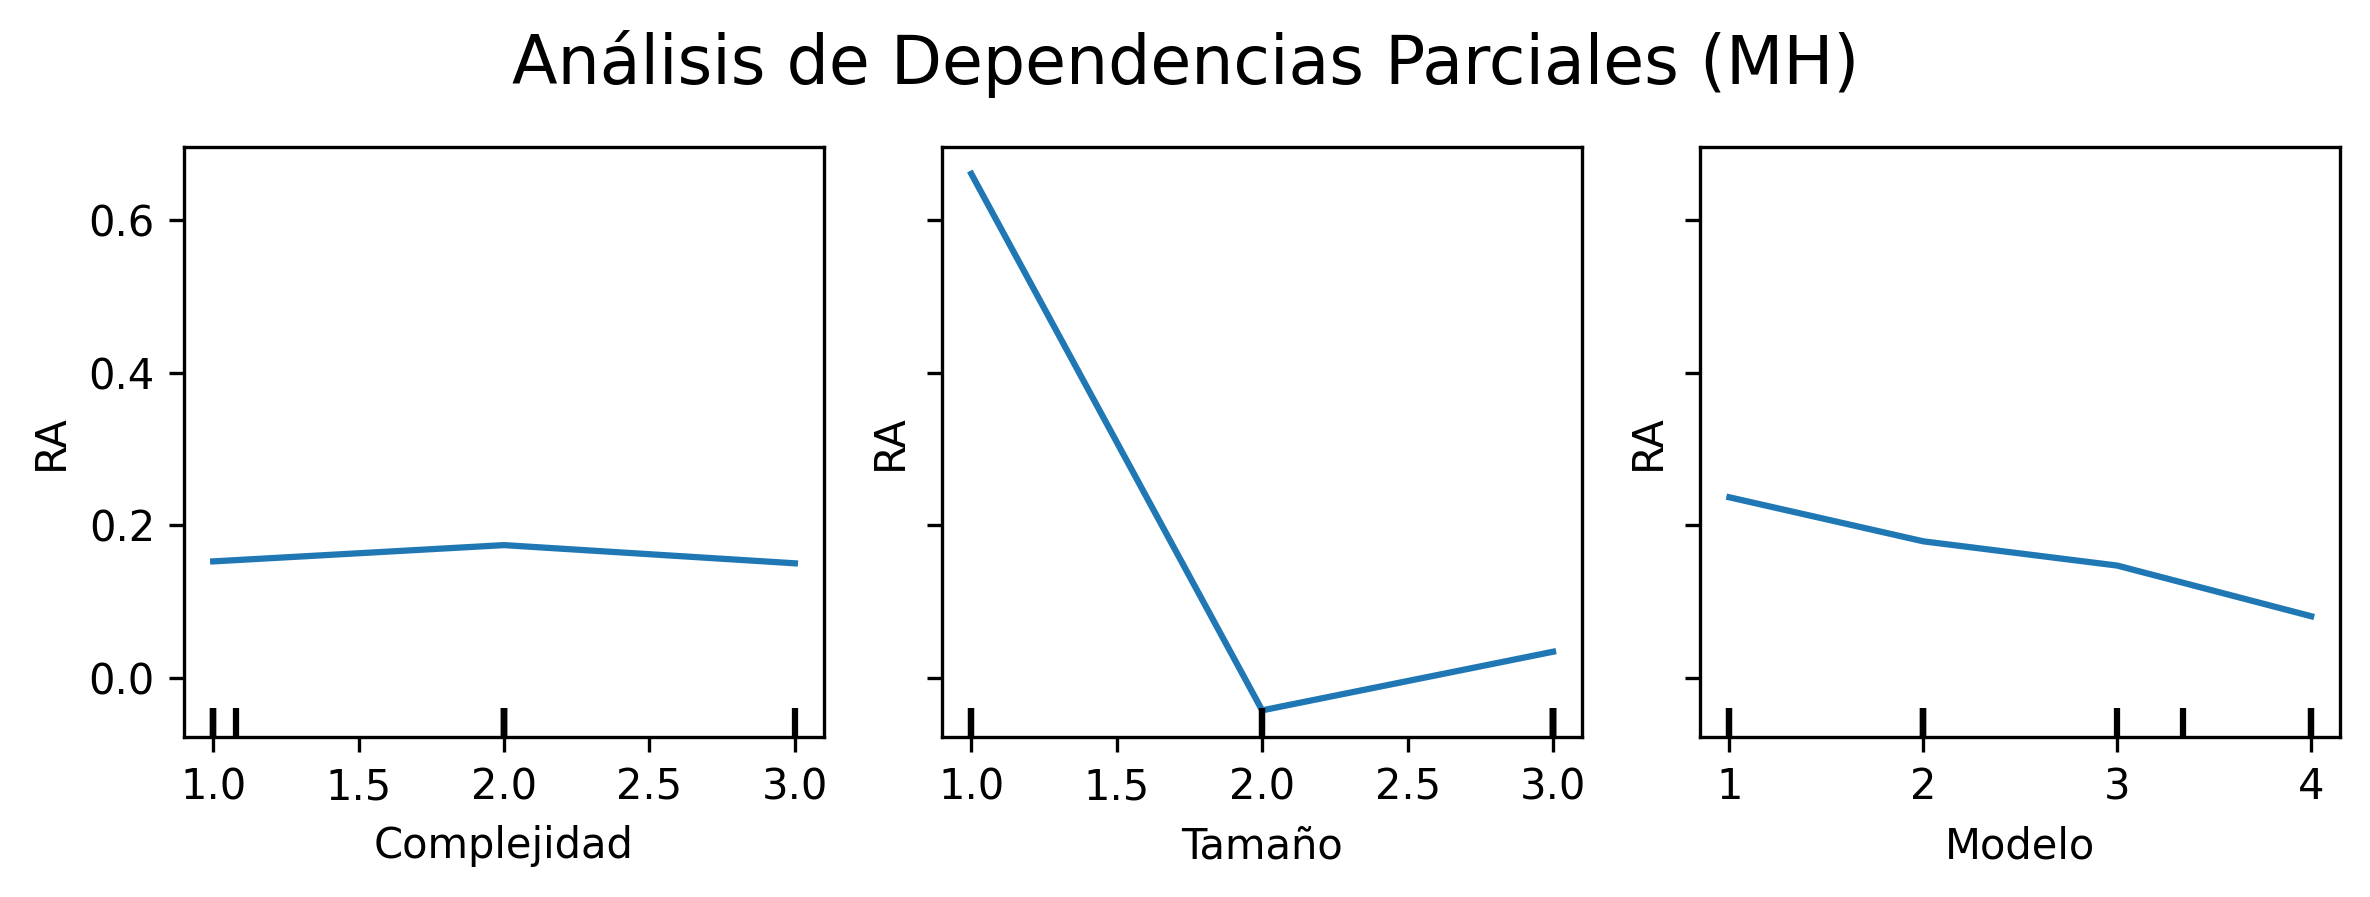
\includegraphics[width=1.0\linewidth]{Plantilla_TFG_latex//imagenes//Inf//Resultados/P1/pda_mh.png}
    \label{fig:pda_mh}}
    \hfill
    \subfloat{ 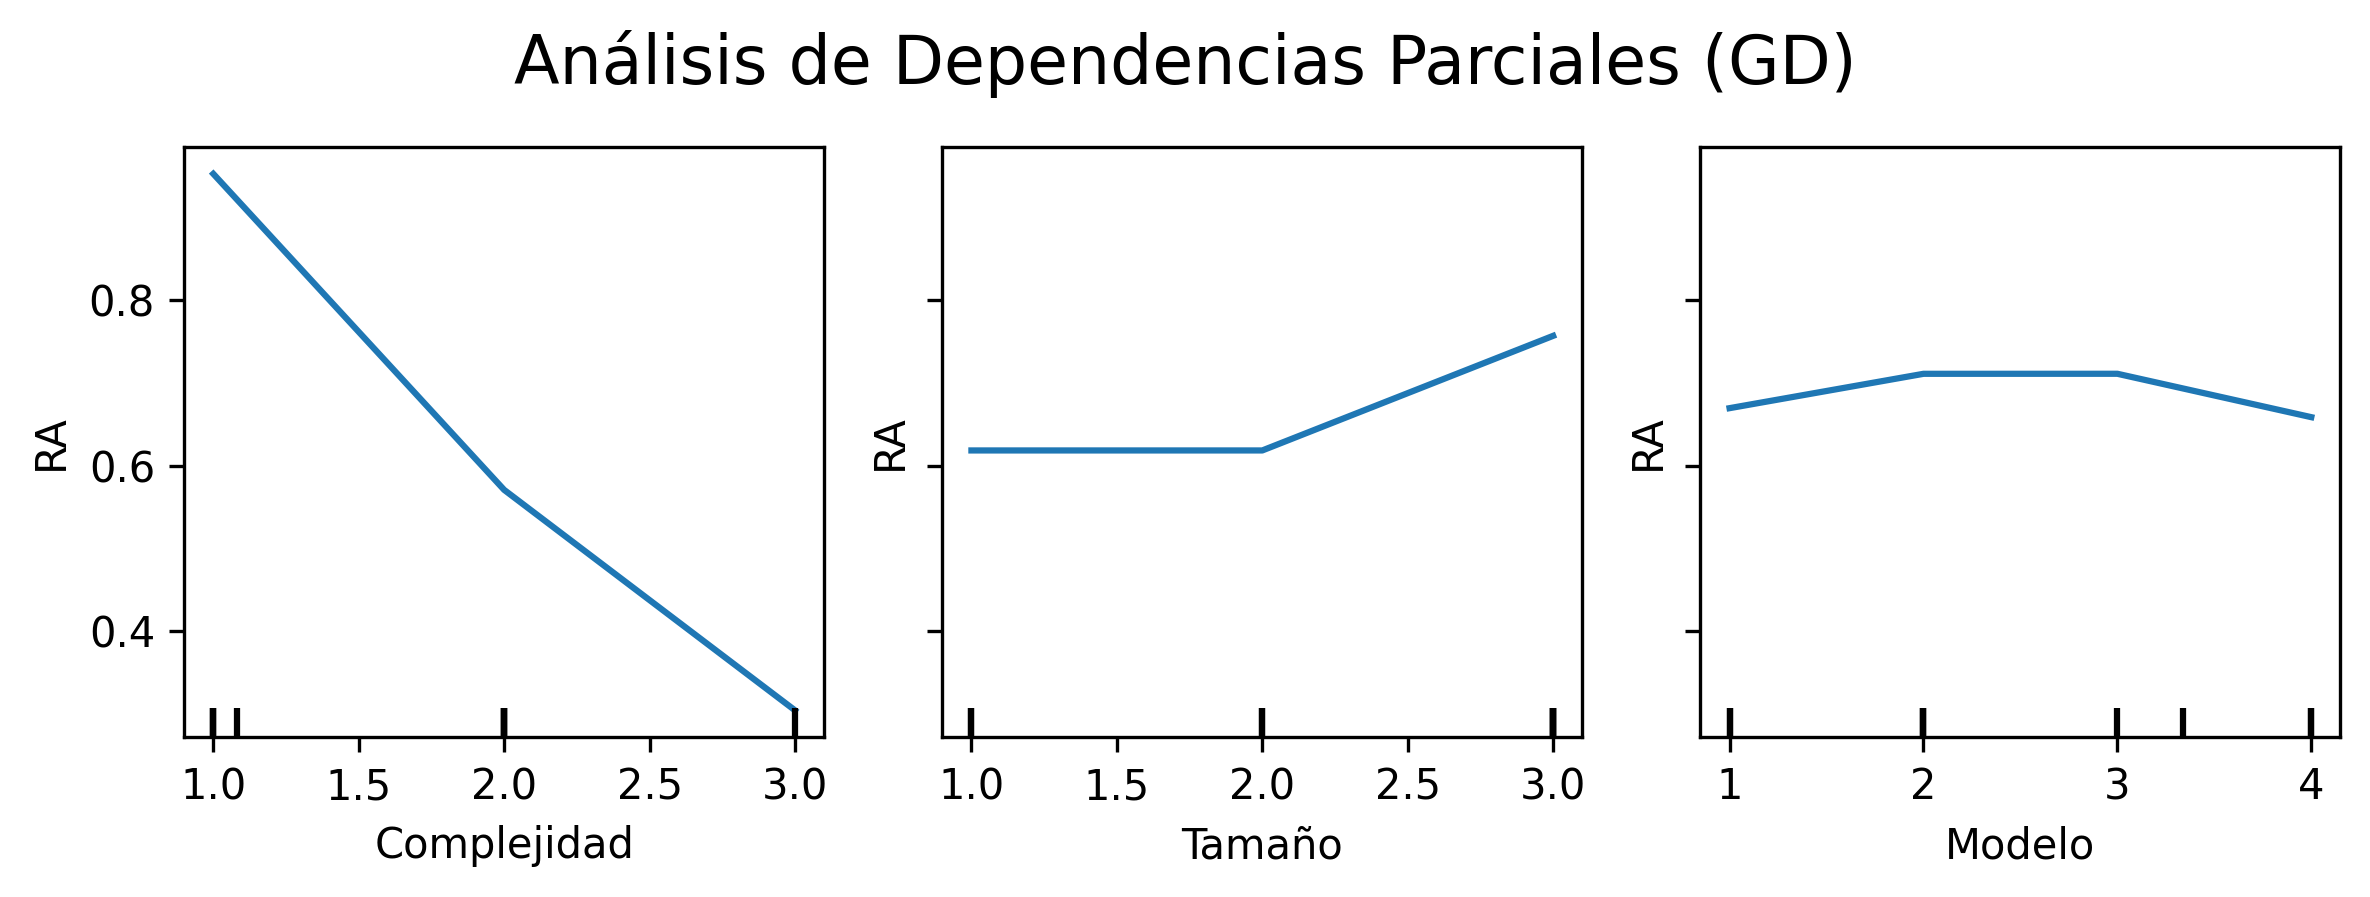
\includegraphics[width=1.0\linewidth]{Plantilla_TFG_latex//imagenes//Inf//Resultados/P1/pda_gd.png}    
    \label{fig:pda_gd}}   
    \caption[Análisis de dependencias parciales del rendimiento relativo al clasificador aleatorio en función de la complejidad del conjunto de datos, el tamaño del conjunto de datos y el número de parámetros del modelo]{Análisis de dependencias parciales del rendimiento relativo al clasificador aleatorio (RA) en función de la complejidad del conjunto de datos, el tamaño del conjunto de datos y el número de parámetros del modelo, para modelos entrenados con AdamW y RMSProp (GD); y SHADE y SHADE-ILS (MH). La primera fila de gráficos muestra los resultados obtenidos con MH, mientras que la segunda corresponde a GD. En cada conjunto de gráficos, el primer panel representa la relación entre la complejidad de la tarea y el RA, el segundo panel muestra el efecto del tamaño del conjunto de datos sobre el RA, y el tercero analiza la influencia del número de parámetros del modelo en el RA. Una tendencia decreciente indica un impacto negativo en el rendimiento, mientras que una tendencia creciente sugiere una mejora en el desempeño del modelo. Se observa que GD es más sensible a la complejidad de la tarea, mientras que MH muestra una caída abrupta en rendimiento con conjuntos de datos más grandes.}
    \label{fig:pda}
\end{figure}




\textbf{En el caso de las MH}, vemos que \textbf{las gráficas correspondientes al tamaño del modelo y la complejidad del conjunto de datos son prácticamente planas}, por lo que concluimos que \textbf{estos dos factores no afectan al rendimiento de los modelos entrenados con técnicas MH}. En contraposición, y contrariamente a la hipótesis planteada, la pendiente correspondiente a \textbf{la cantidad de ejemplos} en el conjunto de datos es muy acusada y negativa, lo que quiere decir que \textbf{este factor influye de manera inversamente proporcional al rendimiento de los modelos. Es decir, cuantos más datos de entrenamiento, peor rinde el modelo.}


\textbf{Con respecto al GD}, tenemos que \textbf{el número de ejemplos y el tamaño del modelo afectan en mucha menor medida que la complejidad de la tarea}. Aunque estos efectos son suaves, podemos observar ciertas tendencias que corroboran lo que conocemos a nivel teórico y verifica la hipótesis planteada. Generalmente, cuantos más ejemplos de entrenamiento tengamos mejor rendimiento tendremos, ya que al tener una muestra mayor los modelos pueden aprender más patrones y más complejos. Por otro lado, sabemos que aumentar el número de parámetros en un modelo no siempre equivale a un mejor rendimiento, y si lo aumentamos sin un criterio concreto podemos caer en un sobreajuste que empeore el rendimiento. Estas ideas pueden observarse de manera leve.

\textbf{Con la complejidad de la tarea sí que se observa una caída brusca de rendimiento conforme ésta crece}. De nuevo corroboramos la literatura y, además, podemos cuantificar y comparar. \textbf{En resumen, para optimizadores basados en GD el incremento de la complejidad de la tarea afecta muy negativamente al rendimiento del modelo}, mientras que el número de parámetros y el número de ejemplos afectan de manera leve, con unas interacciones que deben ser analizadas más minuciosamente. \textbf{En el caso de las MH, es el incremento del número de ejemplos el que contribuye a empeorar rápidamente el rendimiento de los modelos}, mientras que la complejidad del conjunto de datos y el número de parámetros del modelo no afectan prácticamente.






\subsubsection{Experimento 3: Análisis de los tiempos de ejecución en el entrenamiento con MH, tanto en MLPs como en ConvNets}

La hipótesis que planteamos ahora es que \textbf{el tiempo de ejecución de los algoritmos de entrenamiento varía significativamente entre las MH y el GD, siendo las primeras generalmente más costosas computacionalmente}. Específicamente, esperamos que SHADE-ILS tenga un mayor tiempo de ejecución en comparación con AdamW, debido a la naturaleza exploratoria de las metaheurísticas en el espacio de soluciones. Esperamos también que esta diferencia de tiempo tenga como base una ejecución menos optimizada, traducida en mayor tiempo de ejecución por época.

Con la intención de comprender mejor los tiempos de ejecución de ambas estrategias, vamos a comparar los tiempos de los algoritmos SHADE-ILS y AdamW, ya que son dos métodos utilizados en los dos experimentos anteriores y por tanto con los que venimos tratando. Como SHADE forma parte de la ejecución del algoritmo SHADE-ILS, analizaremos también el tiempo del primero a partir del segundo. Las tareas que hemos medido, aprovechando experimentos anteriores, junto con el tiempo de ejecución (en segundos), el número de instancias del conjunto y el número de parámetros del modelo, se pueden observar en la Tabla \ref{tab:tiempos}. En base a estas dos variables mostramos gráficamente el tiempo consumido en la Figura \ref{fig:tiemposgraf}.

\begin{table}[]
\resizebox{\textwidth}{!}{\begin{tabular}{|c|c|c|c|c|c|}
\hline
\textbf{Conjunto} & \textbf{Instancias} & \textbf{Modelo} & \textbf{Tamaño Modelo} & \textbf{SHADE-ILS} & \textbf{AdamW}   \\ \hline
BCW               & 569                 & MLP1            & 2238                   & \textbf{136.436}   & \textbf{2.442}   \\ \hline
BCW               & 569                 & MLP2            & 6462                   & \textbf{147.795}   & \textbf{2.448}   \\ \hline
BCW               & 569                 & MLP5            & 85000                  & \textbf{251.935}   & \textbf{2.611}   \\ \hline
BCW               & 569                 & MLP11           & 1400000                & \textbf{1791.067}  & \textbf{3.103}   \\ \hline
BHP               & 506                 & MLP1            & 2238                   & \textbf{56.217}    & \textbf{1.041}   \\ \hline
BHP               & 506                 & MLP2            & 6462                   & \textbf{61.645}    & \textbf{1.005}   \\ \hline
BHP               & 506                 & MLP5            & 85000                  & \textbf{110.071}   & \textbf{1.197}   \\ \hline
BHP               & 506                 & MLP11           & 1400000                & \textbf{833.789}   & \textbf{1.385}   \\ \hline
WQC               & 4898                & MLP1            & 2238                   & \textbf{800.998}   & \textbf{9.691}   \\ \hline
WQC               & 4898                & MLP2            & 6462                   & \textbf{867.628}   & \textbf{10.065}  \\ \hline
WQC               & 4898                & MLP5            & 85000                  & \textbf{1111.359}  & \textbf{12.283}  \\ \hline
WQC               & 4898                & MLP11           & 1400000                & \textbf{2395.200}  & \textbf{17.922}  \\ \hline
WQR               & 4898                & MLP1            & 2238                   & \textbf{785.936}   & \textbf{9.677}   \\ \hline
WQR               & 4898                & MLP2            & 6462                   & \textbf{856.806}   & \textbf{10.111}  \\ \hline
WQR               & 4898                & MLP5            & 85000                  & \textbf{1123.316}  & \textbf{11.907}  \\ \hline
WQR               & 4898                & MLP11           & 1400000                & \textbf{2054.672}  & \textbf{15.203}  \\ \hline
MNIST             & 15000               & LeNet5          & 62000                  & \textbf{7254.432}  & \textbf{54.999}  \\ \hline
MNIST             & 15000               & ResNet15        & 500000                 & \textbf{7991.074}  & \textbf{61.035}  \\ \hline
MNIST             & 15000               & ResNet57        & 1400000                & \textbf{8785.166}  & \textbf{72.317}  \\ \hline
FMNIST            & 15000               & LeNet5          & 62000                  & \textbf{6068.308}  & \textbf{56.922}  \\ \hline
FMNIST            & 15000               & ResNet15        & 500000                 & \textbf{6735.368}  & \textbf{63.989}  \\ \hline
FMNIST            & 15000               & ResNet57        & 1400000                & \textbf{10914.907} & \textbf{73.486}  \\ \hline
CIFAR             & 15000               & LeNet5          & 62000                  & \textbf{7453.761}  & \textbf{107.512} \\ \hline
CIFAR             & 15000               & ResNet15        & 500000                 & \textbf{8164.679}  & \textbf{113.781} \\ \hline
CIFAR             & 15000               & ResNet57        & 1400000                & \textbf{8812.613}  & \textbf{123.113} \\ \hline
\end{tabular}}
\caption[Comparación de tiempos entre los algoritmos SHADE-ILS y AdamW]{Tabla comparativa que muestra los tiempos de ejecución (en segundos) de los algoritmos SHADE-ILS y AdamW. Se muestra el conjunto de datos con el número de ejemplos correspondiente, además del modelo que se entrena con el número de parámetros que tiene. Se observa un incremento significativo en los tiempos de ejecución de SHADE-ILS con respecto a AdamW conforme aumenta la complejidad y el tamaño de los modelos y/o de los conjuntos de datos.}
\label{tab:tiempos}
\end{table}


\begin{figure}
    \centering
    \subfloat{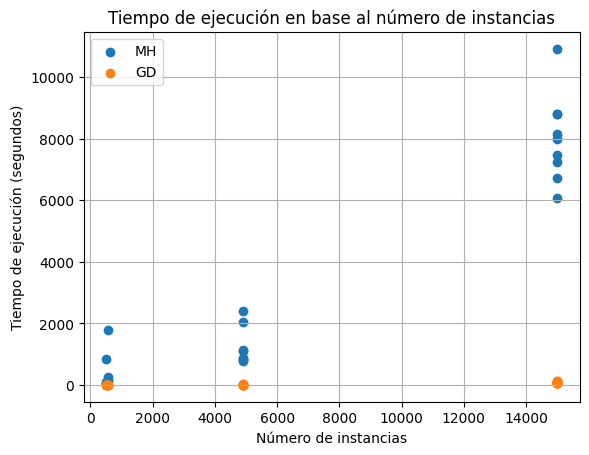
\includegraphics[width=0.85\linewidth]{Plantilla_TFG_latex//imagenes//Inf//Resultados/tiempo/instancias.png}\label{fig:tiempoinst}}
    \hfill
    \subfloat{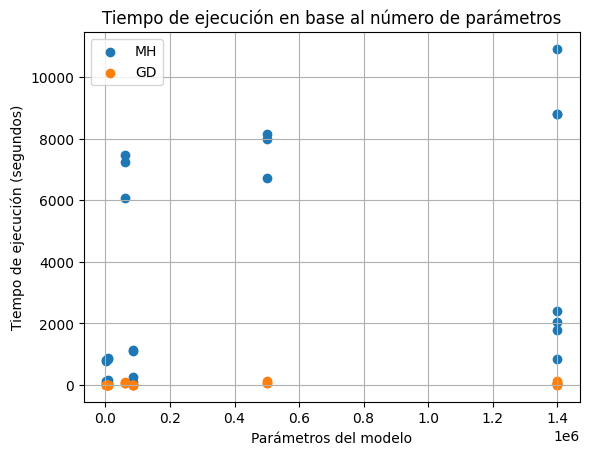
\includegraphics[width=0.85\linewidth]{Plantilla_TFG_latex//imagenes//Inf//Resultados/tiempo/parametros.png}\label{fig:tiempoparam}}
    \caption[Representación gráfica del tiempo de ejecución de los algoritmos SHADE-ILS y AdamW en función del número de parámetros del modelo]{Tiempo de ejecución (en segundos) de SHADE-ILS (MH) y AdamW (GD) en el entrenamiento en función del número de instancias del conjunto de datos (arriba) y del número de parámetros del modelo (abajo). Se observa que SHADE-ILS (azul) presenta tiempos de ejecución considerablemente mayores en comparación con AdamW (naranja), especialmente a medida que aumenta el número de instancias y la cantidad de parámetros del modelo. En particular, el tiempo de ejecución de SHADE-ILS crece de manera pronunciada con ambos factores, especialmente el número de instancias del conjunto de datos.}
    \label{fig:tiemposgraf}
\end{figure}


\begin{figure}
    \centering
    \subfloat{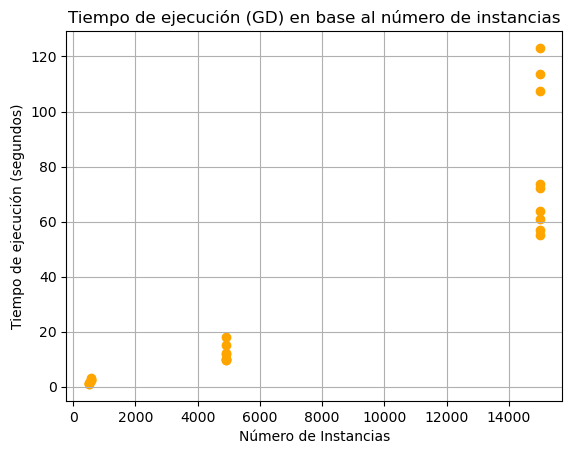
\includegraphics[width=0.85\linewidth]{Plantilla_TFG_latex//imagenes//Inf//Resultados/tiempo/instancias_gd.png}\label{fig:tiempoinst_gd}}
    \hfill
    \subfloat{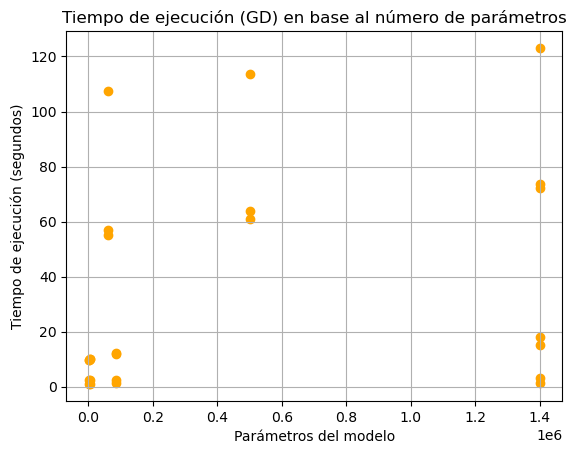
\includegraphics[width=0.85\linewidth]{Plantilla_TFG_latex//imagenes//Inf//Resultados/tiempo/parametros_gd.png}\label{fig:tiempoparam_gd}}
    \caption[Representación gráfica del tiempo de ejecución de AdamW en función del número de parámetros del modelo]{Tiempo de ejecución (en segundos) de AdamW (GD) en el entrenamiento en función del número de instancias del conjunto de datos (arriba) y del número de parámetros del modelo (abajo). Se observa que el número de instancias tiene un efecto mucho mayor que el número de parámetros del modelo.}
    \label{fig:tiemposgraf}
\end{figure}





  

Observando la Figura \ref{fig:tiempoparam}, vemos que la diferencia de tiempos entre algoritmos aumenta en menor medida que en la Figura \ref{fig:tiempoinst}. Además, en la Figura \ref{fig:tiempoparam} existe una amplitud muy grande entre la ejecución más rápida y más lenta del algoritmo SHADE-ILS, variabilidad que viene dada por las ejecuciones con distinto número de instancias, mientras que en la Figura \ref{fig:tiempoinst} los tiempos de las distintas ejecuciones son más compactos. Por tanto podemos afirmar que el número de instancias del conjunto de datos influye más en el tiempo de ejecución de las MH que el número de parámetros del modelo

Vemos clara la lentitud de la opción MH en comparación con la estrategia de GD, vamos pues a analizar de dónde surge esa diferencia y si es esperable a nivel teórico ya que asignamos más ejecuciones a los algoritmos MH. Elegiremos como referencia el caso de FMNIST con el modelo ResNet57. Mientras que SHADE-ILS tarda 10914.907 segundos, AdamW consume 73.486, es decir 148 veces más. Tenemos que tener en cuenta que asignamos más recursos computacionales a la ejecución de SHADE-ILS, pero la diferencia no se corresponde con la teoría. AdamW realiza 20 evaluaciones del conjunto de entrenamiento, mientras que SHADE-ILS hace 4200, 210 veces más. Por lo tanto mejoramos el tiempo que se supone que tendría a nivel teórico.

Observando las figuras \ref{fig:tiempoinst_gd} y\ref{fig:tiempoparam_gd} vemos que el número de ejemplos del conjunto de entrenamiento también tiene mayor peso en el tiempo de ejecución de AdamW, al igual que ocurría en el caso del algoritmo MH. El rango en el que se mueve el número de ejemplos (15 mil) es mucho menor del que se mueve el número de parámetros (1 millón aproximadamente), por lo que \textbf{este tiene un efecto proporcionalmente mucho mayor, del orden de 7 a 10 veces más.}


Vamos a desglosar los tiempos del algoritmo SHADE-ILS para comprenderlo mejor. La función de error propia que hemos implementado para las MH tarda 2.107 segundos en cada evaluación del conjunto de entrenamiento. Como SHADE-ILS ejecuta alrededor de 4200 evaluaciones de las cuales 4000 son realizadas con esa función, en total tenemos que consume 8428 segundos. Las otras 200 evaluaciones se llevan a cabo por el algoritmo de búsqueda local, que consume 4.158 segundos por eje por ejecución, lo que se traduce en un total de 831.600 segundos. Como a nivel abstracto ejecutamos 20 épocas (cada época son 200 evaluaciones de SHADE y 10 de búsqueda local), guardamos un histórico con 20 modelos a los que calculamos el error de validación y \textit{accuracy}, en lo que consumimos 66.400 segundos, que hacen un total de 9326.000 segundos. 

Esa diferencia de tiempo con los 10914.907 segundos totales son principalmente a las funciones de mutación y de cruce. Vamos a suponer que consumen el mismo tiempo y vamos a despreciar otras operaciones secundarias. Como SHADE ejecuta 4000 evaluaciones y tenemos 10 individuos, habrá 400 generaciones, lo que supone 8000 operaciones entre cruces y mutaciones. La diferencia entre el tiempo de la Tabla \ref{tab:tiempos} y el que hemos calculado en el párrafo anterior es de 1588.907 segundos, que si los atribuimos a las operaciones de cruce y mutación tenemos que consumen 0.199 segundos por operación. 

Concluimos por tanto, que \textbf{en términos de tiempo de ejecución por época las MH no son más lentas que el GD, de hecho lo mejoran. Sin embargo necesitan de muchas más ejecuciones para conseguir resultados que puedan asemejarse, en el mejor de los casos, a los obtenidos por optimizadores basados en GD}. Tenemos además un desglose de los tiempos que consumen las funciones que integran el algoritmo SHADE-ILS. La búsqueda local es la que más tiempo consume por ejecución, seguida de la operación de evaluar el conjunto de validación y obtener el valor de \textit{accuracy}, aunque precisamente estas dos últimas operaciones son las que menos se ejecutan. 

Como conclusión final del experimento, obtenemos dos afirmaciones:

\begin{enumerate}

\item El número de instancias del conjunto de datos con el que entrenamos influye más en el tiempo de entrenamiento que el número de parámetros del modelo, del orden de 7 a 10 veces más. Esto ocurre tanto para MH como para GD

\item En términos de tiempo de ejecución por época, las técnicas MH requieren menos tiempo de ejecución que los optimizadores basados en GD, resultado contrario a lo planteado en la hipótesis. Sin embargo, el hecho de que se necesiten muchas más épocas (del orden de 100 o 200 veces más) en las primeras para obtener resultados que se acerquen a las segundas, hace que el tiempo total de ejecución sea mucho mayor en las MH.

\end{enumerate}





%%%%%%%%%%%%%%%%%%%%%%%%%%%%%


\subsubsection{Experimento 4: Análisis comparativo de las propuestas propias} \label{sec:res_propias}



% Please add the following required packages to your document preamble:
% \usepackage{multirow}
\begin{table}[tbp]
\centering
\resizebox{\textwidth}{!}{\begin{tabular}{|c|c|ccc|ccc|}
\hline
\multirow{2}{*}{\textbf{Conjunto}} & \multirow{2}{*}{\textbf{Modelo}} & \multicolumn{3}{c|}{\textbf{SHADE}}                                                         & \multicolumn{3}{c|}{\textbf{SHADE-GD}}                                                                            \\ \cline{3-8} 
                                   &                                  & \multicolumn{1}{c|}{Train}          & \multicolumn{1}{c|}{Test}    & Métrica                & \multicolumn{1}{c|}{Train}            & \multicolumn{1}{c|}{Test}             & Métrica                           \\ \hline
\multirow{4}{*}{BCW}               & 1                                & \multicolumn{1}{c|}{0.112}          & \multicolumn{1}{c|}{0.187}   & \textbf{0.931}         & \multicolumn{1}{c|}{\textbf{0.108}}   & \multicolumn{1}{c|}{\textbf{0.181}}   & 0.915                             \\ \cline{2-8} 
                                   & 2                                & \multicolumn{1}{c|}{0.215}          & \multicolumn{1}{c|}{0.493}   & 0.725                  & \multicolumn{1}{c|}{\textbf{0.118}}   & \multicolumn{1}{c|}{\textbf{0.222}}   & \textbf{0.953}                    \\ \cline{2-8} 
                                   & 5                                & \multicolumn{1}{c|}{0.636}          & \multicolumn{1}{c|}{0.646}   & 0.825                  & \multicolumn{1}{c|}{\textbf{0.106}}   & \multicolumn{1}{c|}{\textbf{0.452}}   & \textbf{0.879}                    \\ \cline{2-8} 
                                   & 11                               & \multicolumn{1}{c|}{0.701}          & \multicolumn{1}{c|}{0.693}   & 0.500                  & \multicolumn{1}{c|}{\textbf{0.279}}   & \multicolumn{1}{c|}{\textbf{0.660}}   & \textbf{0.600}                    \\ \hline
\multirow{4}{*}{WQC}               & 1                                & \multicolumn{1}{c|}{2.100}          & \multicolumn{1}{c|}{2.475}   & \textbf{0.295}         & \multicolumn{1}{c|}{\textbf{1.082}}   & \multicolumn{1}{c|}{\textbf{1.304}}   & 0.171                             \\ \cline{2-8} 
                                   & 2                                & \multicolumn{1}{c|}{2.668}          & \multicolumn{1}{c|}{2.315}   & \textbf{0.214}         & \multicolumn{1}{c|}{\textbf{1.025}}   & \multicolumn{1}{c|}{\textbf{1.486}}   & 0.192                             \\ \cline{2-8} 
                                   & 5                                & \multicolumn{1}{c|}{2.303}          & \multicolumn{1}{c|}{2.304}   & 0.042                  & \multicolumn{1}{c|}{\textbf{0.953}}   & \multicolumn{1}{c|}{\textbf{1.495}}   & \textbf{0.203}                    \\ \cline{2-8} 
                                   & 11                               & \multicolumn{1}{c|}{2.662}          & \multicolumn{1}{c|}{2.302}   & 0.000                  & \multicolumn{1}{c|}{\textbf{1.104}}   & \multicolumn{1}{c|}{\textbf{3.982}}   & \textbf{0.211}                    \\ \hline
\multirow{4}{*}{BHP}               & 1                                & \multicolumn{1}{c|}{430.906}        & \multicolumn{1}{c|}{452.366} & $-1.922 \times 10^{4}$ & \multicolumn{1}{c|}{\textbf{13.977}}  & \multicolumn{1}{c|}{\textbf{33.099}}  & \textbf{0.650}                    \\ \cline{2-8} 
                                   & 2                                & \multicolumn{1}{c|}{430.970}        & \multicolumn{1}{c|}{428.226} & $-9.607 \times 10^{2}$ & \multicolumn{1}{c|}{\textbf{384.431}} & \multicolumn{1}{c|}{\textbf{128.808}} & \textbf{-4.610}                   \\ \cline{2-8} 
                                   & 5                                & \multicolumn{1}{c|}{429.719}        & \multicolumn{1}{c|}{435.000} & $-7.318 \times 10^{3}$ & \multicolumn{1}{c|}{\textbf{396.344}} & \multicolumn{1}{c|}{\textbf{324.056}} & \textbf{-0.932}                   \\ \cline{2-8} 
                                   & 11                               & \multicolumn{1}{c|}{469.788}        & \multicolumn{1}{c|}{454.786} & $-5.381 \times 10^{6}$ & \multicolumn{1}{c|}{\textbf{463.336}} & \multicolumn{1}{c|}{\textbf{453.891}} & \textbf{-1.294 $\times$ 10$^{5}$} \\ \hline
\multirow{4}{*}{WQR}               & 1                                & \multicolumn{1}{c|}{34.645}         & \multicolumn{1}{c|}{34.336}  & $-4.150 \times 10^{2}$ & \multicolumn{1}{c|}{\textbf{0.622}}   & \multicolumn{1}{c|}{\textbf{0.712}}   & \textbf{-2.624}                   \\ \cline{2-8} 
                                   & 2                                & \multicolumn{1}{c|}{35.425}         & \multicolumn{1}{c|}{30.956}  & $-2.020 \times 10^{3}$ & \multicolumn{1}{c|}{\textbf{0.562}}   & \multicolumn{1}{c|}{\textbf{1.548}}   & \textbf{-0.442}                   \\ \cline{2-8} 
                                   & 5                                & \multicolumn{1}{c|}{34.767}         & \multicolumn{1}{c|}{32.230}  & $-2.135 \times 10^{5}$ & \multicolumn{1}{c|}{\textbf{0.568}}   & \multicolumn{1}{c|}{\textbf{0.934}}   & \textbf{-3.447}                   \\ \cline{2-8} 
                                   & 11                               & \multicolumn{1}{c|}{\textbf{35.867}}         & \multicolumn{1}{c|}{32.176}  & $-1.951 \times 10^{6}$ & \multicolumn{1}{c|}{35.937}  & \multicolumn{1}{c|}{\textbf{32.039}}  & \textbf{-2.312 $\times$ 10$^{5}$} \\ \hline
\multirow{3}{*}{MNIST}             & LeNet5                           & \multicolumn{1}{c|}{2.424}          & \multicolumn{1}{c|}{2.277}   & 0.171                  & \multicolumn{1}{c|}{\textbf{0.110}}   & \multicolumn{1}{c|}{\textbf{1.930}}   & \textbf{0.529}                    \\ \cline{2-8} 
                                   & ResNet15                         & \multicolumn{1}{c|}{2.811}          & \multicolumn{1}{c|}{2.302}   & 0.100                  & \multicolumn{1}{c|}{\textbf{0.408}}   & \multicolumn{1}{c|}{2.301}            & 0.100                             \\ \cline{2-8} 
                                   & ResNet57                         & \multicolumn{1}{c|}{3.639}          & \multicolumn{1}{c|}{2.302}   & 0.082                  & \multicolumn{1}{c|}{\textbf{2.730}}   & \multicolumn{1}{c|}{2.302}            & \textbf{0.120}                    \\ \hline
\multirow{3}{*}{F-MNIST}           & LeNet5                           & \multicolumn{1}{c|}{1.498}          & \multicolumn{1}{c|}{2.291}   & 0.180                  & \multicolumn{1}{c|}{\textbf{0.705}}   & \multicolumn{1}{c|}{\textbf{2.140}}   & \textbf{0.360}                    \\ \cline{2-8} 
                                   & ResNet15                         & \multicolumn{1}{c|}{\textbf{2.668}} & \multicolumn{1}{c|}{2.303}   & 0.104                  & \multicolumn{1}{c|}{3.547}            & \multicolumn{1}{c|}{2.302}            & 0.100                             \\ \cline{2-8} 
                                   & ResNet57                         & \multicolumn{1}{c|}{2.525}          & \multicolumn{1}{c|}{2.303}   & 0.100                  & \multicolumn{1}{c|}{\textbf{1.389}}   & \multicolumn{1}{c|}{2.303}            & 0.100                             \\ \hline
\multirow{3}{*}{CIFAR-10G}        & LeNet5                           & \multicolumn{1}{c|}{2.548}          & \multicolumn{1}{c|}{2.300}   & 0.102                  & \multicolumn{1}{c|}{\textbf{1.483}}   & \multicolumn{1}{c|}{\textbf{2.275}}   & \textbf{0.142}                    \\ \cline{2-8} 
                                   & ResNet15                         & \multicolumn{1}{c|}{\textbf{2.536}} & \multicolumn{1}{c|}{2.303}   & \textbf{0.111}         & \multicolumn{1}{c|}{2.798}            & \multicolumn{1}{c|}{2.303}            & 0.096                             \\ \cline{2-8} 
                                   & ResNet57                         & \multicolumn{1}{c|}{2.723}          & \multicolumn{1}{c|}{2.303}   & 0.099                  & \multicolumn{1}{c|}{\textbf{2.701}}   & \multicolumn{1}{c|}{2.303}            & 0.093                             \\ \hline
\end{tabular}}
\caption[Comparación del desempeño de SHADE y SHADE-GD en el entrenamiento de modelos de aprendizaje profundo sobre conjuntos de datos tabulares e imágenes]{Comparación del desempeño de SHADE y SHADE-GD en el entrenamiento de modelos de aprendizaje profundo sobre conjuntos de datos tabulares e imágenes. Se presentan los errores de entrenamiento (\textit{Train}) y evaluación (\textit{Test}), junto con la métrica de desempeño utilizada en cada caso (\textbf{\textit{Balanced Accuracy}} para BCW y WQC, \textbf{\emph{R$^2$}}  para BHP y WQR, y \textbf{\textit{accuracy}} para MNIST, Fashion-MNIST y CIFAR-10 en escala de grises). Para datos tabulares, se emplean modelos MLP con distintas profundidades, mientras que para imágenes se evalúan modelos de la familia ConvNet (LeNet5, ResNet15 y ResNet57)  (columna Modelo). Los valores resaltados indican el mejor desempeño en cada caso. En las filas sin valores resaltados, ambos métodos presentan un rendimiento equivalente. Consideramos que el modelo con mejor rendimiento es el que tiene mejor valor en su métrica. Se observa que SHADE-GD generalmente supera a SHADE, especialmente en modelos más profundos y en conjuntos de datos tabulares, donde SHADE tiende a deteriorarse.}
\label{tab:shadevsshadegd}
\end{table}






\vspace{0.4cm}
\paragraph{SHADE y SHADE-GD\\}  


\mbox{}
\vspace{0.1cm}

Comentamos los resultados obtenidos del entrenamiento y que se muestran en la Tabla \ref{tab:shadevsshadegd}. SHADE-GD supera a SHADE en la mayoría de los escenarios, logrando menores errores en entrenamiento y prueba. La incorporación del descenso de gradiente mejora la optimización de los pesos, reduciendo el sobreajuste y favoreciendo la generalización. En contraste, SHADE muestra inconsistencias a medida que aumenta la complejidad del modelo, con errores significativamente mayores en entornos de alta dimensionalidad.

SHADE sufre mayor deterioro en la generalización, especialmente en modelos profundos y conjuntos de datos grandes como MNIST y CIFAR-10G, donde sus métricas de desempeño son muy bajas. SHADE-GD, en cambio, reduce la pérdida en entrenamiento sin aumentar drásticamente la pérdida en prueba, evitando estancamientos en soluciones subóptimas.

SHADE muestra un deterioro progresivo en arquitecturas con mayor número de parámetros, con un rendimiento deficiente en modelos MLP con 5 y 11 capas ocultas, así como en redes convolucionales complejas como ResNet15 y ResNet57. SHADE-GD mantiene un desempeño más estable y presenta mejoras en redes convolucionales, aunque persisten dificultades en modelos profundos.

\textbf{En clasificación, SHADE-GD obtiene mejores métricas, especialmente en modelos simples} como LeNet5, aunque sigue sin igualar métodos basados en gradientes en modelos más complejos. En regresión, SHADE muestra valores extremadamente negativos en $R^2$, mientras que SHADE-GD logra métricas más aceptables, destacando su ventaja en la minimización del error.

SHADE-GD sigue sin ser competitivo en redes profundas aplicadas a conjuntos de datos complejos como CIFAR-10G, posiblemente debido a una exploración inicial ineficiente en SHADE. Además, SHADE tiende a estancarse en soluciones subóptimas cuando la dimensionalidad del espacio de búsqueda es alta, resultando en métricas de evaluación deficientes.

\textbf{Como conclusión, SHADE-GD supera a SHADE en la mayoría de los casos, mostrando menor error y mejor desempeño, aunque aún enfrenta limitaciones en redes profundas y conjuntos de datos grandes}. Se requieren estrategias adicionales de optimización para mejorar su eficacia en escenarios más complejos.




% Please add the following required packages to your document preamble:
% \usepackage{multirow}
\begin{table}[tbp]
\resizebox{\textwidth}{!}{\begin{tabular}{|c|c|ccc|ccc|}
\hline
\multirow{2}{*}{\textbf{Conjunto}} & \multirow{2}{*}{\textbf{Modelo}} & \multicolumn{3}{c|}{\textbf{SHADE-ILS}}                                                            & \multicolumn{3}{c|}{\textbf{SHADE-ILS-GD}}                                                                    \\ \cline{3-8} 
                                   &                                  & \multicolumn{1}{c|}{Train}          & \multicolumn{1}{c|}{Test}           & Métrica                & \multicolumn{1}{c|}{Train}           & \multicolumn{1}{c|}{Test}            & Métrica                         \\ \hline
\multirow{4}{*}{BCW}               & 1                                & \multicolumn{1}{c|}{0.073}          & \multicolumn{1}{c|}{\textbf{0.142}} & \textbf{0.970}         & \multicolumn{1}{c|}{\textbf{0.062}}  & \multicolumn{1}{c|}{0.159}           & 0.941                           \\ \cline{2-8} 
                                   & 2                                & \multicolumn{1}{c|}{0.063}          & \multicolumn{1}{c|}{0.350}          & 0.932                  & \multicolumn{1}{c|}{0.063}           & \multicolumn{1}{c|}{0.350}           & 0.932                           \\ \cline{2-8} 
                                   & 5                                & \multicolumn{1}{c|}{0.055}          & \multicolumn{1}{c|}{\textbf{0.475}} & \textbf{0.891}         & \multicolumn{1}{c|}{\textbf{0.031}}  & \multicolumn{1}{c|}{0.616}           & 0.600                           \\ \cline{2-8} 
                                   & 11                               & \multicolumn{1}{c|}{\textbf{0.099}} & \multicolumn{1}{c|}{\textbf{0.491}} & \textbf{0.903}         & \multicolumn{1}{c|}{0.112}           & \multicolumn{1}{c|}{0.704}           & 0.500                           \\ \hline
\multirow{4}{*}{WQC}               & 1                                & \multicolumn{1}{c|}{1.098}          & \multicolumn{1}{c|}{1.235}          & 0.201                  & \multicolumn{1}{c|}{\textbf{1.068}}  & \multicolumn{1}{c|}{\textbf{1.224}}  & \textbf{0.226}                  \\ \cline{2-8} 
                                   & 2                                & \multicolumn{1}{c|}{1.078}          & \multicolumn{1}{c|}{1.340}          & 0.167                  & \multicolumn{1}{c|}{\textbf{1.065}}  & \multicolumn{1}{c|}{\textbf{1.400}}  & \textbf{0.306}                  \\ \cline{2-8} 
                                   & 5                                & \multicolumn{1}{c|}{0.963}          & \multicolumn{1}{c|}{1.405}          & 0.167                  & \multicolumn{1}{c|}{\textbf{0.951}}  & \multicolumn{1}{c|}{\textbf{1.328}}  & 0.166                           \\ \cline{2-8} 
                                   & 11                               & \multicolumn{1}{c|}{1.138}          & \multicolumn{1}{c|}{1.509}          & 0.167                  & \multicolumn{1}{c|}{\textbf{1.099}}  & \multicolumn{1}{c|}{\textbf{1.496}}  & 0.167                           \\ \hline
\multirow{4}{*}{BHP}               & 1                                & \multicolumn{1}{c|}{10.048}         & \multicolumn{1}{c|}{7.549}          & 0.576                  & \multicolumn{1}{c|}{\textbf{8.928}}  & \multicolumn{1}{c|}{\textbf{3.895}}  & \textbf{0.849}                  \\ \cline{2-8} 
                                   & 2                                & \multicolumn{1}{c|}{9.561}          & \multicolumn{1}{c|}{4.649}          & 0.747                  & \multicolumn{1}{c|}{9.561}           & \multicolumn{1}{c|}{4.649}           & 0.747                           \\ \cline{2-8} 
                                   & 5                                & \multicolumn{1}{c|}{13.594}         & \multicolumn{1}{c|}{14.556}         & -0.187                 & \multicolumn{1}{c|}{\textbf{11.689}} & \multicolumn{1}{c|}{\textbf{14.368}} & \textbf{-0.078}                 \\ \cline{2-8} 
                                   & 11                               & \multicolumn{1}{c|}{43.184}         & \multicolumn{1}{c|}{26.794}         & -97.405                & \multicolumn{1}{c|}{43.184}          & \multicolumn{1}{c|}{26.794}          & -97.405                         \\ \hline
\multirow{4}{*}{WQR}               & 1                                & \multicolumn{1}{c|}{0.611}          & \multicolumn{1}{c|}{0.970}          & -1.987                 & \multicolumn{1}{c|}{\textbf{0.599}}  & \multicolumn{1}{c|}{\textbf{0.912}}  & \textbf{-1.898}                 \\ \cline{2-8} 
                                   & 2                                & \multicolumn{1}{c|}{0.579}          & \multicolumn{1}{c|}{0.826}          & -2.491                 & \multicolumn{1}{c|}{\textbf{0.521}}  & \multicolumn{1}{c|}{\textbf{0.620}}  & \textbf{-4.105}                 \\ \cline{2-8} 
                                   & 5                                & \multicolumn{1}{c|}{0.589}          & \multicolumn{1}{c|}{\textbf{0.724}} & -9.832 $\times$ 10$^2$ & \multicolumn{1}{c|}{\textbf{0.579}}  & \multicolumn{1}{c|}{0.747}           & \textbf{-2.347 $\times$ 10$^2$} \\ \cline{2-8} 
                                   & 11                               & \multicolumn{1}{c|}{0.601}          & \multicolumn{1}{c|}{\textbf{0.734}} & -7.953 $\times$ 10$^4$ & \multicolumn{1}{c|}{0.601}           & \multicolumn{1}{c|}{0.774}           & -7.953 $\times$ 10$^{4}$        \\ \hline
\multirow{3}{*}{MNIST}             & LeNet5                           & \multicolumn{1}{c|}{2.530}          & \multicolumn{1}{c|}{2.300}          & 0.066                  & \multicolumn{1}{c|}{2.530}           & \multicolumn{1}{c|}{2.300}           & 0.066                           \\ \cline{2-8} 
                                   & ResNet15                         & \multicolumn{1}{c|}{0.001}          & \multicolumn{1}{c|}{2.294}          & \textbf{0.115}         & \multicolumn{1}{c|}{0.001}           & \multicolumn{1}{c|}{2.292}           & 0.100                           \\ \cline{2-8} 
                                   & ResNet57                         & \multicolumn{1}{c|}{2.308}          & \multicolumn{1}{c|}{2.303}          & 0.100                  & \multicolumn{1}{c|}{\textbf{0.001}}  & \multicolumn{1}{c|}{2.303}           & 0.100                           \\ \hline
\multirow{3}{*}{F-MNIST}           & LeNet5                           & \multicolumn{1}{c|}{0.403}          & \multicolumn{1}{c|}{1.807}          & 0.366                  & \multicolumn{1}{c|}{\textbf{0.327}}  & \multicolumn{1}{c|}{\textbf{1.646}}  & \textbf{0.462}                  \\ \cline{2-8} 
                                   & ResNet15                         & \multicolumn{1}{c|}{3.547}          & \multicolumn{1}{c|}{2.302}          & \textbf{0.100}         & \multicolumn{1}{c|}{\textbf{0.349}}  & \multicolumn{1}{c|}{2.302}           & 0.063                           \\ \cline{2-8} 
                                   & ResNet57                         & \multicolumn{1}{c|}{2.673}          & \multicolumn{1}{c|}{2.303}          & 0.100                  & \multicolumn{1}{c|}{\textbf{1.208}}  & \multicolumn{1}{c|}{2.303}           & 0.100                           \\ \hline
\multirow{3}{*}{CIFAR-10G}        & LeNet5                           & \multicolumn{1}{c|}{2.568}          & \multicolumn{1}{c|}{2.301}          & 0.114                  & \multicolumn{1}{c|}{2.568}           & \multicolumn{1}{c|}{2.301}           & 0.114                           \\ \cline{2-8} 
                                   & ResNet15                         & \multicolumn{1}{c|}{\textbf{1.697}} & \multicolumn{1}{c|}{2.303}          & \textbf{0.103}         & \multicolumn{1}{c|}{3.504}           & \multicolumn{1}{c|}{2.303}           & 0.093                           \\ \cline{2-8} 
                                   & ResNet57                         & \multicolumn{1}{c|}{2.579}          & \multicolumn{1}{c|}{2.303}          & \textbf{0.100}         & \multicolumn{1}{c|}{\textbf{2.415}}  & \multicolumn{1}{c|}{2.303}           & 0.096                           \\ \hline
\end{tabular}}
\caption[Comparación del desempeño de SHADE-ILS y SHADE-ILS-GD en el entrenamiento de modelos de aprendizaje profundo sobre conjuntos de datos tabulares e imágenes]{Comparación del desempeño de SHADE-ILS y SHADE-ILS-GD en el entrenamiento de modelos de aprendizaje profundo sobre conjuntos de datos tabulares e imágenes. Se presentan los errores de entrenamiento (\textit{Train}) y evaluación (\textit{Test}), junto con la métrica de desempeño utilizada en cada caso (\textit{Balanced Accuracy} para BCW y WQC, $R^2$  para BHP y WQR, y \textit{accuracy} para MNIST, Fashion-MNIST y CIFAR-10 en escala de grises). Para datos tabulares, se emplean modelos MLP con distintas profundidades, mientras que para imágenes se evalúan modelos de la familia ConvNet (LeNet5, ResNet15 y ResNet57)  (columna Modelo). Los valores resaltados indican el mejor desempeño en cada caso. En las filas sin valores resaltados, ambos métodos presentan un rendimiento equivalente. Consideramos que el modelo con mejor rendimiento es el que tiene mejor valor en su métrica. No hay una diferencia clara entre ambos optimizadores, aunque se observa que SHADE-ILS en su versión original consigue más robustez, siendo más estable en la mayoría de tareas.}
\label{tab:ilsvsilsgd}
\end{table}

\vspace{0.4cm}
\paragraph{SHADE-ILS y SHADE-ILS-GD\\} 

\mbox{}
\vspace{0.1cm}


Comentamos los resultados obtenidos del entrenamiento y que se muestran en la Tabla \ref{tab:ilsvsilsgd}. El rendimiento de SHADE-ILS y SHADE-ILS-GD varía según la complejidad del problema y la arquitectura de la red utilizada. Aunque SHADE-ILS-GD puede reducir el error en algunos casos, no siempre mejora la capacidad de generalización del modelo. En redes profundas y conjuntos de datos de mayortamaño,\textbf{ la combinación con GD no siempre aporta ventajas significativas sobre SHADE-ILS}.

\textbf{SHADE-ILS muestra mayor estabilidad en modelos profundos}, donde la introducción de GD en SHADE-ILS-GD a menudo induce fluctuaciones en la convergencia. En particular, en la tarea de clasificación sobre un conjunto de datos con alta dimensionalidad, SHADE-ILS-GD presentó variaciones bruscas en el valor de la métrica entre iteraciones, mientras que SHADE-ILS mantuvo una convergencia más uniforme. En tareas de regresión tabular, SHADE-ILS-GD mostró mejoras esporádicas en el coeficiente $R^2$, pero también una mayor propensión al sobreajuste cuando se aumentó la cantidad de capas en la red.

\textbf{En problemas de regresión, SHADE-ILS-GD mejora la generalización en redes poco profundas}, como en el caso de un modelo de tres capas donde redujo el error de evaluación en un 7\% (Tabla \ref{tab:ilsvsilsgd}). Sin embargo, \textbf{en redes más complejas, esta ventaja desaparece}, e incluso el modelo entrenado con SHADE-ILS mantiene un desempeño más estable en el conjunto de entrenamiento. En clasificación, SHADE-ILS-GD no muestra mejoras consistentes y, en algunos casos, como en MNIST, obtuvo un valor de \textit{accuracy} 3\% inferior a la de SHADE-ILS. En modelos convolucionales aplicados a conjuntos de datos de imágenes, SHADE-ILS-GD rara vez aporta mejoras y, en ocasiones, introduce sobreajuste, como se evidenció en una prueba donde el error de entrenamiento disminuyó sin que la métrica en el conjunto de prueba mejorara.

\textbf{Como conclusión, SHADE-ILS es una opción más eficiente y estable en redes profundas, mientras que SHADE-ILS-GD puede aportar mejoras en regresión con arquitecturas simples}. Sin embargo, el refinamiento con GD no garantiza una mejor generalización y puede inducir sobreajuste o aumentar significativamente el tiempo de cómputo sin beneficios claros. En datos tabulares, SHADE-ILS-GD presenta mejoras ocasionales, pero en imágenes y redes profundas, SHADE-ILS sigue siendo la alternativa más confiable. Estos resultados sugieren que la incorporación de GD en SHADE-ILS debe evaluarse caso por caso, ya que sus beneficios no son universales y dependen del tipo de tarea y arquitectura utilizada.



% Please add the following required packages to your document preamble:
% \usepackage{multirow}
\begin{table}[tbp]
\resizebox{\textwidth}{!}{\begin{tabular}{|c|c|ccc|ccc|}
\hline
\multirow{2}{*}{\textbf{Conjunto}} & \multirow{2}{*}{\textbf{Modelo}} & \multicolumn{3}{c|}{\textbf{SHADE-GD}}                                                               & \multicolumn{3}{c|}{\textbf{SHADE-ILS-GD}}                                                                      \\ \cline{3-8} 
                                   &                                  & \multicolumn{1}{c|}{Train}          & \multicolumn{1}{c|}{Test}           & Métrica                  & \multicolumn{1}{c|}{Train}           & \multicolumn{1}{c|}{Test}            & Métrica                           \\ \hline
\multirow{4}{*}{BCW}               & 1                                & \multicolumn{1}{c|}{0.108}          & \multicolumn{1}{c|}{0.181}          & 0.915                    & \multicolumn{1}{c|}{\textbf{0.062}}  & \multicolumn{1}{c|}{\textbf{0.159}}  & \textbf{0.941}                    \\ \cline{2-8} 
                                   & 2                                & \multicolumn{1}{c|}{0.118}          & \multicolumn{1}{c|}{\textbf{0.222}} & \textbf{0.953}           & \multicolumn{1}{c|}{\textbf{0.063}}  & \multicolumn{1}{c|}{0.350}           & 0.932                             \\ \cline{2-8} 
                                   & 5                                & \multicolumn{1}{c|}{0.106}          & \multicolumn{1}{c|}{\textbf{0.452}} & \textbf{0.879}           & \multicolumn{1}{c|}{\textbf{0.031}}  & \multicolumn{1}{c|}{0.616}           & 0.600                             \\ \cline{2-8} 
                                   & 11                               & \multicolumn{1}{c|}{0.279}          & \multicolumn{1}{c|}{\textbf{0.660}} & \textbf{0.600}           & \multicolumn{1}{c|}{\textbf{0.112}}  & \multicolumn{1}{c|}{0.704}           & 0.500                             \\ \hline
\multirow{4}{*}{WQC}               & 1                                & \multicolumn{1}{c|}{1.082}          & \multicolumn{1}{c|}{1.304}          & 0.171                    & \multicolumn{1}{c|}{\textbf{1.068}}  & \multicolumn{1}{c|}{\textbf{1.224}}  & \textbf{0.226}                    \\ \cline{2-8} 
                                   & 2                                & \multicolumn{1}{c|}{\textbf{1.025}} & \multicolumn{1}{c|}{1.486}          & 0.192                    & \multicolumn{1}{c|}{1.065}           & \multicolumn{1}{c|}{\textbf{1.400}}  & \textbf{0.306}                    \\ \cline{2-8} 
                                   & 5                                & \multicolumn{1}{c|}{0.953}          & \multicolumn{1}{c|}{1.495}          & \textbf{0.203}           & \multicolumn{1}{c|}{0.951}           & \multicolumn{1}{c|}{\textbf{1.328}}  & 0.166                             \\ \cline{2-8} 
                                   & 11                               & \multicolumn{1}{c|}{1.104}          & \multicolumn{1}{c|}{3.982}          & \textbf{0.211}           & \multicolumn{1}{c|}{\textbf{1.099}}  & \multicolumn{1}{c|}{\textbf{1.496}}  & 0.167                             \\ \hline
\multirow{4}{*}{BHP}               & 1                                & \multicolumn{1}{c|}{13.977}         & \multicolumn{1}{c|}{33.099}         & 0.650                    & \multicolumn{1}{c|}{\textbf{8.928}}  & \multicolumn{1}{c|}{\textbf{3.895}}  & \textbf{0.849}                    \\ \cline{2-8} 
                                   & 2                                & \multicolumn{1}{c|}{384.431}        & \multicolumn{1}{c|}{128.808}        & -4.610                   & \multicolumn{1}{c|}{\textbf{9.561}}  & \multicolumn{1}{c|}{\textbf{4.649}}  & \textbf{0.747}                    \\ \cline{2-8} 
                                   & 5                                & \multicolumn{1}{c|}{396.344}        & \multicolumn{1}{c|}{324.056}        & -0.932                   & \multicolumn{1}{c|}{\textbf{11.689}} & \multicolumn{1}{c|}{\textbf{14.368}} & \textbf{-0.078}                   \\ \cline{2-8} 
                                   & 11                               & \multicolumn{1}{c|}{463.336}        & \multicolumn{1}{c|}{453.891}        & -1.294 $\times$ 10$^{5}$ & \multicolumn{1}{c|}{\textbf{43.184}} & \multicolumn{1}{c|}{\textbf{26.794}} & \textbf{-97.405}                  \\ \hline
\multirow{4}{*}{WQR}               & 1                                & \multicolumn{1}{c|}{0.622}          & \multicolumn{1}{c|}{\textbf{0.712}} & -2.624                   & \multicolumn{1}{c|}{\textbf{0.599}}  & \multicolumn{1}{c|}{0.912}           & \textbf{-1.898}                   \\ \cline{2-8} 
                                   & 2                                & \multicolumn{1}{c|}{0.562}          & \multicolumn{1}{c|}{1.548}          & \textbf{-0.442}          & \multicolumn{1}{c|}{\textbf{0.521}}  & \multicolumn{1}{c|}{\textbf{0.620}}  & -4.105                            \\ \cline{2-8} 
                                   & 5                                & \multicolumn{1}{c|}{\textbf{0.568}} & \multicolumn{1}{c|}{0.934}          & \textbf{-3.447}          & \multicolumn{1}{c|}{0.579}           & \multicolumn{1}{c|}{\textbf{0.747}}  & -2.347 $\times$ 10$^2$            \\ \cline{2-8} 
                                   & 11                               & \multicolumn{1}{c|}{35.937}         & \multicolumn{1}{c|}{32.039}         & -2.312 $\times$ 10$^{5}$ & \multicolumn{1}{c|}{\textbf{0.601}}  & \multicolumn{1}{c|}{\textbf{0.774}}  & \textbf{-7.953 $\times$ 10$^{4}$} \\ \hline
\multirow{3}{*}{MNIST}             & LeNet5                           & \multicolumn{1}{c|}{\textbf{0.110}} & \multicolumn{1}{c|}{\textbf{1.930}} & \textbf{0.529}           & \multicolumn{1}{c|}{2.530}           & \multicolumn{1}{c|}{2.300}           & 0.066                             \\ \cline{2-8} 
                                   & ResNet15                         & \multicolumn{1}{c|}{0.408}          & \multicolumn{1}{c|}{\textbf{2.301}} & 0.100                    & \multicolumn{1}{c|}{\textbf{0.001}}  & \multicolumn{1}{c|}{2.292}           & 0.100                             \\ \cline{2-8} 
                                   & ResNet57                         & \multicolumn{1}{c|}{2.730}          & \multicolumn{1}{c|}{2.302}          & \textbf{0.120}           & \multicolumn{1}{c|}{\textbf{0.001}}  & \multicolumn{1}{c|}{2.303}           & 0.100                             \\ \hline
\multirow{3}{*}{F-MNIST}           & LeNet5                           & \multicolumn{1}{c|}{0.705}          & \multicolumn{1}{c|}{2.140}          & 0.360                    & \multicolumn{1}{c|}{\textbf{0.327}}  & \multicolumn{1}{c|}{\textbf{1.646}}  & \textbf{0.462}                    \\ \cline{2-8} 
                                   & ResNet15                         & \multicolumn{1}{c|}{3.547}          & \multicolumn{1}{c|}{2.302}          & \textbf{0.100}           & \multicolumn{1}{c|}{\textbf{0.349}}  & \multicolumn{1}{c|}{2.302}           & 0.063                             \\ \cline{2-8} 
                                   & ResNet57                         & \multicolumn{1}{c|}{1.389}          & \multicolumn{1}{c|}{2.303}          & 0.100                    & \multicolumn{1}{c|}{\textbf{1.208}}  & \multicolumn{1}{c|}{2.303}           & 0.100                             \\ \hline
\multirow{3}{*}{CIFAR-10G}        & LeNet5                           & \multicolumn{1}{c|}{\textbf{1.483}} & \multicolumn{1}{c|}{\textbf{2.275}} & \textbf{0.142}           & \multicolumn{1}{c|}{2.568}           & \multicolumn{1}{c|}{2.301}           & 0.114                             \\ \cline{2-8} 
                                   & ResNet15                         & \multicolumn{1}{c|}{\textbf{2.798}} & \multicolumn{1}{c|}{2.303}          & 0.096                    & \multicolumn{1}{c|}{3.504}           & \multicolumn{1}{c|}{2.303}           & 0.093                             \\ \cline{2-8} 
                                   & ResNet57                         & \multicolumn{1}{c|}{2.701}          & \multicolumn{1}{c|}{2.303}          & 0.093                    & \multicolumn{1}{c|}{\textbf{2.415}}  & \multicolumn{1}{c|}{2.303}           & 0.096                             \\ \hline
\end{tabular}}
\caption[Comparación del desempeño de SHADE-GD y SHADE-ILS-GD en el entrenamiento de modelos de aprendizaje profundo sobre conjuntos de datos tabulares e imágenes]{Comparación del desempeño de SHADE-ILS y SHADE-ILS-GD en el entrenamiento de modelos de aprendizaje profundo sobre conjuntos de datos tabulares e imágenes. Se presentan los errores de entrenamiento (\textit{Train}) y evaluación (\textit{Test}), junto con la métrica de desempeño utilizada en cada caso (\textit{Balanced Accuracy} para BCW y WQC, $R^2$  para BHP y WQR, y \textit{accuracy} para MNIST, Fashion-MNIST y CIFAR-10 en escala de grises). Para datos tabulares, se emplean modelos MLP con distintas profundidades, mientras que para imágenes se evalúan modelos de la familia ConvNet (LeNet5, ResNet15 y ResNet57)  (columna Modelo). Los valores resaltados indican el mejor desempeño en cada caso. En las filas sin valores resaltados, ambos métodos presentan un rendimiento equivalente. Consideramos que el modelo con mejor rendimiento es el que tiene mejor valor en su métrica. Aunque no hay una diferencia clara entre los dos optimizadores, existe un patrón reconocible, en el que se evidencia que SHADE-GD tiende a generalizar mejor mientras que SHADE-ILS-GD minimiza más la función de pérdida.}
\label{tab:shadegdvsilsgd}
\end{table}

\vspace{0.4cm}
\paragraph{SHADE-GD y SHADE-ILS-GD\\} 

\mbox{}
\vspace{0.1cm}

\textbf{En términos generales, SHADE-ILS-GD muestra un mejor rendimiento en los conjuntos de datos más complejos o con mayor variabilidad}. En particular, destaca en el conjunto BHP, donde logra mejoras sustanciales en las métricas de evaluación. Por ejemplo, en el modelo MLP1, el error en el conjunto de prueba se reduce drásticamente de 33.099 con SHADE-GD a 3.895 con SHADE-ILS-GD, lo que se traduce en un incremento significativo en la métrica de evaluación (de 0.650 a 0.849). Este patrón se repite en otros modelos de BHP, donde SHADE-GD presenta errores elevados mientras que SHADE-ILS-GD los mantiene controlados, incluso revirtiendo resultados negativos.

En los conjuntos de datos de clasificación como BCW y WQC, el comportamiento de ambos algoritmos es más equilibrado, con ventajas alternadas en función del modelo específico. Por ejemplo, en BCW, SHADE-ILS-GD logra mejores resultados en los primeros modelos (e.g., modelo 1 con una métrica de 0.941 frente a 0.915), pero en modelos más complejos como MLP5 y el MLP11, su rendimiento disminuye notablemente en comparación con SHADE-GD. Por otro lado, en WQC, SHADE-ILS-GD tiene una ligera ventaja en la mayoría de los casos, con métricas más altas y errores de prueba más bajos en tres de los cuatro modelos.

En los conjuntos de imágenes como MNIST, F-MNIST y CIFAR-10G, SHADE-GD tiende a ofrecer un rendimiento más consistente en los modelos más simples, especialmente con arquitecturas como LeNet5. Por ejemplo, en MNIST con LeNet5, SHADE-GD alcanza una mejor métrica (0.529 frente a 0.066 de SHADE-ILS-GD) con menores errores en el conjunto de prueba. Sin embargo, en arquitecturas más profundas como ResNet57, ambos algoritmos muestran dificultades para lograr un desempeño óptimo, con métricas cercanas a 0.100 en múltiples instancias.

\textbf{Un patrón recurrente es que SHADE-ILS-GD presenta un mejor ajuste en el conjunto de entrenamiento}, lo que indica una mayor capacidad de minimizar el error durante la optimización. No obstante, \textbf{esta ventaja no siempre se traduce en un mejor rendimiento en el conjunto de prueba, sugiriendo una posible tendencia al sobreajuste} en ciertos modelos y conjuntos de datos. Por el contrario, \textbf{SHADE-GD ofrece una generalización más estable en tareas de clasificación simples}, aunque con dificultades evidentes en casos más complejos como BHP y ciertos modelos en WQR.

\textbf{En resumen, SHADE-ILS-GD destaca por su capacidad de optimización en problemas complejos, particularmente en tareas de regresión con alto error, mientras que SHADE-GD ofrece un rendimiento más equilibrado y generalizable en tareas de clasificación}. La elección entre ambos algoritmos depende en gran medida de la naturaleza del problema: SHADE-ILS-GD es más eficiente para reducir errores en entrenamientos difíciles, mientras que SHADE-GD es más fiable para obtener resultados consistentes en problemas de menor complejidad. En definitiva,\textbf{ es un resultado parejo, aunque consideramos ganador a SHADE-GD} ya que generaliza mejor y consigue mejor métrica en 11 tareas frente a las 10 en las que lo hace SHADE-ILS-GD.